\chapter*{Anhang}\addcontentsline{toc}{chapter}{Anhang}
\section*{Gantt-Diagramm}

\begin{figure}[H]
	\centering
	\includegraphics[width=1.0\linewidth]{images/gantt-diagramm.pdf}
	\caption[Gantt-Diagramm]{Gantt-Diagramm}
	\label{fig:gantt-diagramm}
\end{figure}


\section*{Projektstrukturplan}
\begin{figure}[H]
	\centering
	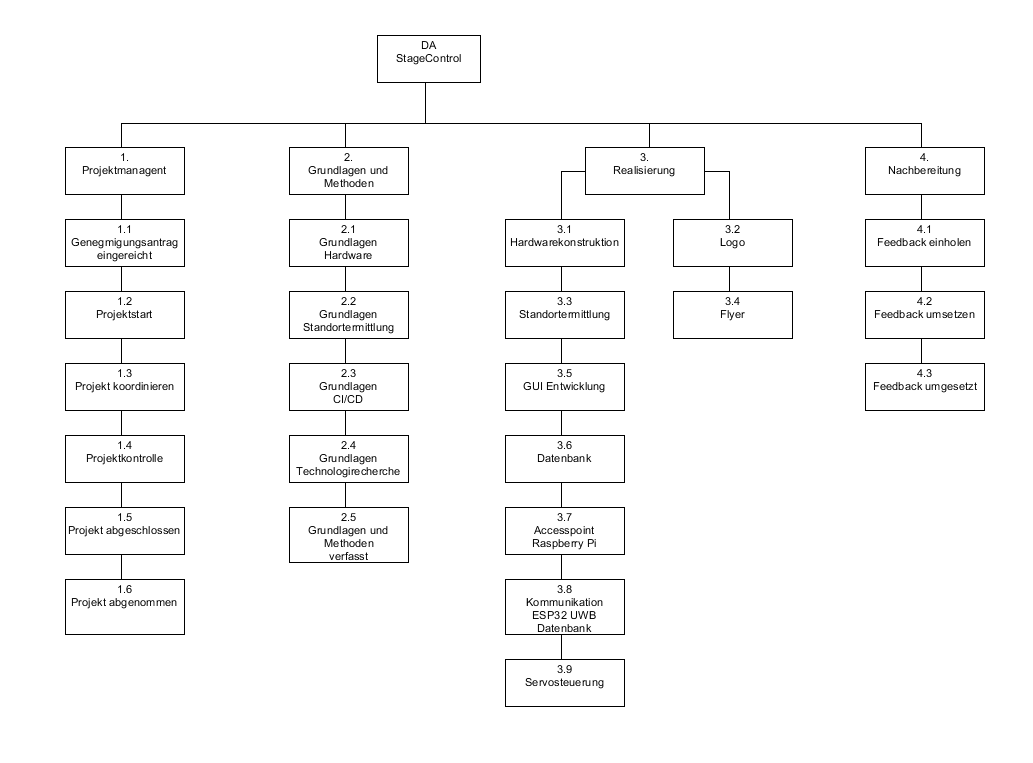
\includegraphics[width=1.0\linewidth]{images/PSP.png}
	\caption[Projektstrukturplan]{Projektstrukturplan}
	\label{fig:projektstrukturplan}
\end{figure}
\newpage

\section*{Meilensteine}
\begin{table}[h]
	\centering
	\begin{tabular}{p{3cm} p{7cm} p{2cm} p{2cm}}
		\hline
		\textbf{PSP-Code} & \textbf{Name} & \textbf{Soll-Datum} & \textbf{Ist-Datum} \\
		\hline
		3.1 & Hardwarekonstruktion & 23.12.2024 & 04.03.2025 \\
		3.2 & Logo & 16.09.2024  & 10.03.2025 \\
		3.3 & Standortermittlung & 31.01.025 & 13.03.2025 \\
		3.4 & Flyer & 20.12.2024 & 07.01.2025 \\
		3.5 & GUI Entwicklung & 30.12.2024 & 28.02.25 \\
		3.6 & Datenbank & 17.12.2024 & 05.01.2025 \\
		3.7 & Access-Point Raspberry Pi & 20.01.2025 & 05.01.2025 \\
		3.8 & Kommunikation ESP32 UWB Datenbank & 23.12.2024  & 08.01.2025 \\
		3.9 & Servosteuerung & 31.01.2025 & 10.03.2025 \\
		\hline
	\end{tabular}
	\caption{Meilensteinliste}
	\label{tab:Meilensteinliste}
\end{table}
\newpage

\section*{Stundenlisten}
In den nachfolgenden Tabellen sind die Stundenlisten pro Monat der einzelnen Mitglieder von StageControl aufgelistet.

\section*{Michael Becksteiner}

\begin{table}[h]
	\begin{tabular}{p{2.5cm} p{10.5cm} p{2.5cm}}
		\hline
		\textbf{Monat} & \textbf{Tätigkeit} & \textbf{Aufwand in Stunden} \\
		\hline
		03.2024 & Aufbau der DA, Themenfindung & 6 \\
		05.2024 & Themenfindung, Genehmigungsverfahren & 5 \\
		06.2024 & Genehmigungsantrag, Namensfindung & 3,2 \\
		07.2024 & LaTeX Projekt aufsetzten& 12 \\
		08.2024 & Grundlagen und Methoden & 11,7 \\
		10.2024 & GUI Entwicklung & 34 \\
		12.2024 & Verbindung GUI - Datenbank - RaspberryPi & 20,4 \\
		02.2025 & ESP32 UWB Anchor und Tag Navigation & 45 \\
		02.2025 & Testphase & 30 \\
		02.2025 &Ergebnisdokumentation & 17 \\
		
		\hline
		\textbf{Summe} & & \textbf{184,3} \\
		\hline
	\end{tabular}
	\caption{Stundenliste Michael Becksteiner}
	\label{tab:arbeitsaufwand_Becksteiner}
\end{table}

\newpage
\section*{Carina Pospichal}
\begin{table}[h]
	\begin{tabular}{p{2.5cm} p{10.5cm} p{2.5cm}}
		\hline
		\textbf{Monat} & \textbf{Tätigkeit} & \textbf{Aufwand in Stunden} \\
		\hline
		03.2024 & Aufbau der DA, Themenfindung & 6 \\
		05.2024 & Themenfindung, Genehmigungsverfahren & 5 \\
		06.2024 & Genehmigungsantrag, Namensfindung & 3,2 \\
		07.2024 & LaTeX Projekt aufsetzten& 12 \\
		08.2024 & Grundlagen und Methoden & 15,6 \\
		09.2024 & Logo & 10,2 \\
		11.2024 & Plaung und Umsetzung Flyer & 35 \\
		12.2024 & Datenbank aufsetzten & 14,7 \\
		01.2025 & Netzwerk Raspberry Pi & 6 \\
		01.2025 & SD-Kartensicherungskopie & 3 \\
		01.2025 & Planung und Umsetzung Logo-Animation & 4 \\
		01.2025 & Statische IPs auf Raspberry Pi einrichten & 5 \\
		02.2025 & Ergebnisdokumentation &  36\\
		02.2025 & Testphase & 30 \\
		
		\hline
		\textbf{Summe} & & \textbf{185,7} \\
		\hline
	\end{tabular}
	\caption{Stundenliste Carina Pospichal}
	\label{tab:arbeitsaufwand_Pospichal}
\end{table}

\newpage

\section*{Leo Pirringer}

\begin{table}[h]
	\begin{tabular}{p{2.5cm} p{10.5cm} p{3cm}}
		\hline
		\textbf{Monat} & \textbf{Tätigkeit} & \textbf{Aufwand in Stunden} \\
		\hline
		03.2024 & Aufbau der DA, Themenfindung & 6 \\
		05.2024 & Themenfindung, Genehmigungsverfahren & 5 \\
		06.2024 & Genehmigungsantrag, Namensfindung & 3,2 \\
		07.2024 & LaTeX Projekt aufsetzten& 12 \\
		08.2024 & Grundlagen und Methoden & 35 \\
		10.2024 & Gerüstbau und Aufsatz Servomotoren & 44,3 \\
		11.2024 & 3D Prototyping und Druck Servo Aufsatz & 35 \\
		02.2025 & Servosteuerung Code & 20 \\
		02.2025 & ESP32 UWB Gehäuse Prototyping und Druck& 15\\
		02.2025 & Ergebnisdokumentation &  20\\
		02.2025 & Testphase & 30 \\
		
		\hline
		\textbf{Summe} & & \textbf{225,5} \\
		\hline
	\end{tabular}
	\caption{Stundenliste Leo Pirringer}
	\label{tab:arbeitsaufwand_Pirringer}
\end{table}